\documentclass[11pt,fleqn]{article}
\usepackage{../cs70,epsf,amsmath,graphicx}

\lecture{9}
\def\title{Note \the\lecturenumber}
\begin{document}
\maketitle

\iffalse
\title{Note 8}
\begin{document}
\maketitle
\fi
%%\stackrel{\smallcirc}{\wedge}}
\section*{Error Correcting Codes}


We will consider two situations in which we wish to transmit
information on an unreliable channel. The first is exemplified by the
internet, where the information (say a file) is broken up into
packets, and the unreliability is manifest in the fact that some of
the packets are lost (or erased) during transmission. Moreover the 
packets are labeled so that the recipient knows exactly which 
packets were received and which were dropped. We will refer to such errors as erasure errors. 
See the figure below:

\includegraphics*[scale=0.70]{erasure.png}

In the second situation, some of the packets are
corrupted during transmission due to channel noise. Now the recipient has no idea which 
packets were corrupted and which were received unmodified:

\includegraphics*[scale=0.70]{general.png}

In the above example, packets 1 and 4 are corrupted. These types of errors are called general errors. We will discuss
methods of encoding messages, called error correcting codes, which are 
capable of correcting both erasure
and general errors.

Assume that the information consists of $n$ packets.
We can assume without loss of generality that the contents of each packet
is a number modulo $q$ (denoted by $GF(q)$), where $q$ is a prime. For example, the contents 
of the packet might be a $32$-bit string 
and can therefore be regarded as a number between $0$ and $2^{32} -1$;
then we could choose $q$ to be any prime larger than $2^{32}$.
The properties of polynomials over $GF(q)$ (i.e., with coefficients 
and values reduced modulo $q$) are the backbone of both error-correcting schemes. To see this, 
let us denote the
message to be sent by $m_1 , \ldots, m_n$ and make the following crucial observations:

\noindent
{\bf 1)} There is a unique polynomial $P(x)$ of degree $n - 1$ such that
$P(i) = m_i$ for $1 \leq i \leq n$ (i.e., $P(x)$ contains all of the information
about the message, and evaluating $P(i)$ gives the contents of the $i$-$th$ packet).

\noindent
{\bf 2)} The message to be sent is now $m_1 = P(1), \ldots, m_n = P(n)$. 
We can generate additional packets by evaluating $P(x)$ at 
additional points $n+1, n+2, \ldots, n+j$ (remember, our transmitted message must be redundant, i.e., it must contain more packets than the original message to account for the lost 
or corrupted packets). Thus the transmitted message is 
$c_1 = P(1) , c_2 = P(2) , \ldots , c_{n+j} = P(n+j)$. Since we 
are working modulo $q$, we must make sure that $n + j \leq q$, but 
this condition does not impose a serious constraint since $q$ is 
very large. 

\subsection*{Erasure Errors}
Here we consider the setting of packets being transmitted over the internet.
In this setting, the packets are labeled and so the recipient knows exactly 
which packets were dropped during transmission. One additional observation
will be useful:

\noindent
{\bf 3)} By Property 2 in Note 8, we can uniquely reconstruct $P(x)$ from its values at any $n$ 
distinct points, since it has degree $n-1$. This means that $P(x)$ 
can be reconstructed from any $n$ of the transmitted packets. Evaluating 
this reconstructed polynomial $P(x)$ at $x = 1, \ldots , n$ yields 
the original message $m_1 , \ldots , m_n$. 

Recall that in our scheme, the transmitted message is 
$c_1 = P(1) , c_2 = P(2) , \ldots , c_{n+j} = P(n+j)$. 
Thus, if we hope to be able to correct $k$ errors, we simply need to set $j= k$.
The encoded message will then consist of $n + k$ packets.  

\subsubsection*{Example}

Suppose Alice wants to send Bob a message of $n=4$ packets and she wants to guard
against $k=2$ lost packets.  Then, assuming the packets can be coded up as integers
between~0 and~6, Alice can work over $GF(7)$ (since $7\ge n+k = 6$).
Suppose the message that Alice wants to send to Bob is 
$m_1 = 3$, $m_2 = 1$, $m_3 = 5$, and $m_4 = 0$.
She interpolates to find the unique polynomial of degree $n - 1 = 3$ described by these 4 points: 
$P(x) = x^3 + 4x^2 + 5$
(verify that $P(i) = m_i$ for $1 \leq i \leq 4$). 

Since $k=2$, Alice must evaluate $P(x)$ at $2$ extra points: 
$P(5) = 6$ and $P(6) = 1$. Now, Alice can transmit the encoded message 
which consists of $n + k = 6$ packets, where $c_j = P(j)$ for $1\leq j \leq 6$. So
$c_1 = P(1) = 3$, $c_2 = P(2) = 1$, $c_3 = P(3) = 5$, $c_4 = P(4) = 0$, $c_5 = P(5) = 6$, 
and $c_6 = P(6) = 1$.  Suppose packets $2$ and $6$ are dropped, 
in which case we have the following situation:

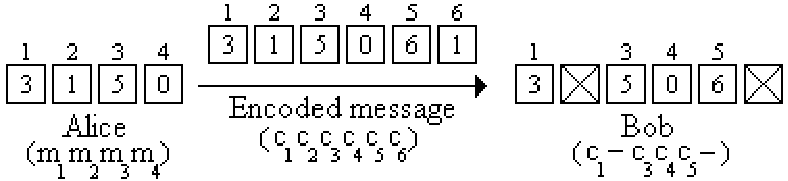
\includegraphics[bb = 0 0 250 87, scale = 0.8]{packets2}

\noindent From the values that Bob received (3, 5, 0, and 6), he uses Lagrange interpolation and computes the following delta functions:
\begin{align*}
\Delta_1(x) &= \frac{(x - 3)(x - 4)(x - 5)}{-24}\\
\Delta_3(x) &= \frac{(x - 1)(x - 4)(x - 5)}{4}\\
\Delta_4(x) &= \frac{(x - 1)(x - 3)(x - 5)}{-3}\\
\Delta_5(x) &= \frac{(x - 1)(x - 3)(x - 4)}{8}.
\end{align*}
He then reconstructs the polynomial $P(x) = (3)\Delta_1(x)+(5)\Delta_3(x)+(0)\Delta_4(x) +
(6)\Delta_5(x) = x^3 + 4x^2 + 5$.
Bob then evaluates $m_2 = P(2) = 1$, which is the packet that was lost from the original 
message.  More generally, no matter which two packets were dropped,
following the same method Bob could still have reconstructed
$P(x)$ and thus the original message.

Let us consider what would happen if Alice sent one fewer packet. If Alice 
only sent $c_j$ for $1 \leq j \leq n + k - 1$, then with
$k$ erasures, Bob would only receive $c_j$ for $n - 1$ distinct values
$j$. Thus, Bob would not be able to reconstruct $P(x)$ (since there are
exactly $q$ polynomials of degree at most $n - 1$ that agree with the $n - 1$ packets
which Bob received). This error-correcting scheme is therefore optimal: it can recover
the $n$ characters of the transmitted message from any $n$ received characters,
but recovery from any fewer characters is impossible.

\subsection*{Polynomial Interpolation}
Let us take a brief digression to discuss another method of 
polynomial interpolation which will be useful in handling general errors. The goal
of the algorithm will be to take as input $d+1$ pairs $(x_1,y_1),\cdots,(x_{d+1},y_{d+1})$,
and output the polynomial $p(x) = a_dx^d + \dots + 
a_1x + a_0$ such that $p(x_i) = y_i$ for $i = 1$ to $d+1$. 

The first step of the algorithm is to write a system of $d+1$ linear equations
in $d+1$ variables: the coefficients of the polynomial $a_0, \ldots, a_d$.
Each equation is obtained by fixing $x$ to be one of $d+1$ values: $x_1,\cdots,x_{d+1}$. Note that in $p(x)$,
$x$ is a variable and $a_0,\dots,a_d$ are fixed constants. In the equations below, these roles are swapped:
$x_i$ is a fixed constant and $a_0,\dots,a_d$ are variables. For example, the $i$-$th$ equation
 is the result of fixing $x$ to be $x_i$:
$a_d x_i^d + a_{d-1} x_i^{d-1} + \ldots + a_0 = y_i$.

Now solving these equations gives the coefficients of the
polynomial $p(x)$. 
For example, given the $3$ pairs $(-1,2)$, $(0,1)$, and $(2,5)$, we will
construct the degree $2$ polynomial $p(x)$ which goes through these points. The first
equation says $a_2(-1)^2 + a_1(-1) + a_0 = 2$. Simplifying, we get $a_2 - a_1 + a_0 = 2$.
Similarly, the second equation says $a_2(0)^2 + a_1(0) + a_0 = 1$, or $a_0 = 1$. 
And the third equation says $a_2(2)^2 + a_1(2) + a_0 = 5$
So we get the following system of equations:
\begin{align*}
a_2 - a_1 + a_0 &= 2\\
a_0 &= 1\\
4a_2 + 2a_1 + a_0 &= 5
\end{align*}
Substituting for $a_0$ and multiplying the first equation by $2$ we get:
\begin{align*}
2a_2 - 2a_1 &= 2\\
4a_2 + 2a_1 &= 4
\end{align*}
Then, adding the two equations we find that $6a_2 = 6$, so $a_2 = 1$, and plugging
back in we find that $a_1 = 0$. Thus, we have determined the polynomial
$p(x) = x^2 + 1$. To justify this method more carefully, we must show that
the equations always have a solution and that it is unique.
This involves showing that a certain determinant is non-zero, which we will leave
as an exercise.
\subsection*{General Errors}
Now let us return to general errors. 
General errors are much more challenging to correct than erasure errors. 
This is because packets are corrupted, not erased and Bob no longer knows
which packets are correct. As we shall see shortly, 
Alice can still guard against $k$ general errors, at the
expense of transmitting only $2k$ additional packets or characters (only
twice as many as in the erasure case). 
Thus the encoded message is $c_1, \ldots, c_{n+2k}$ where
$c_j = P(j)$ for $1 \leq j \leq n + 2k$. This means that at least $n+k$ of these characters are received
uncorrupted by Bob. 


For example, if Alice wishes
to send $n = 4$ characters to Bob via a modem in which $k = 1$ of the characters is corrupted,
she must redundantly send an encoded message consisting of 6 characters. Suppose
she wants to transmit the same message as above, and that $c_1$ is corrupted
and changed to $r_1 = 2$. This scenario can be visualized in the following figure:

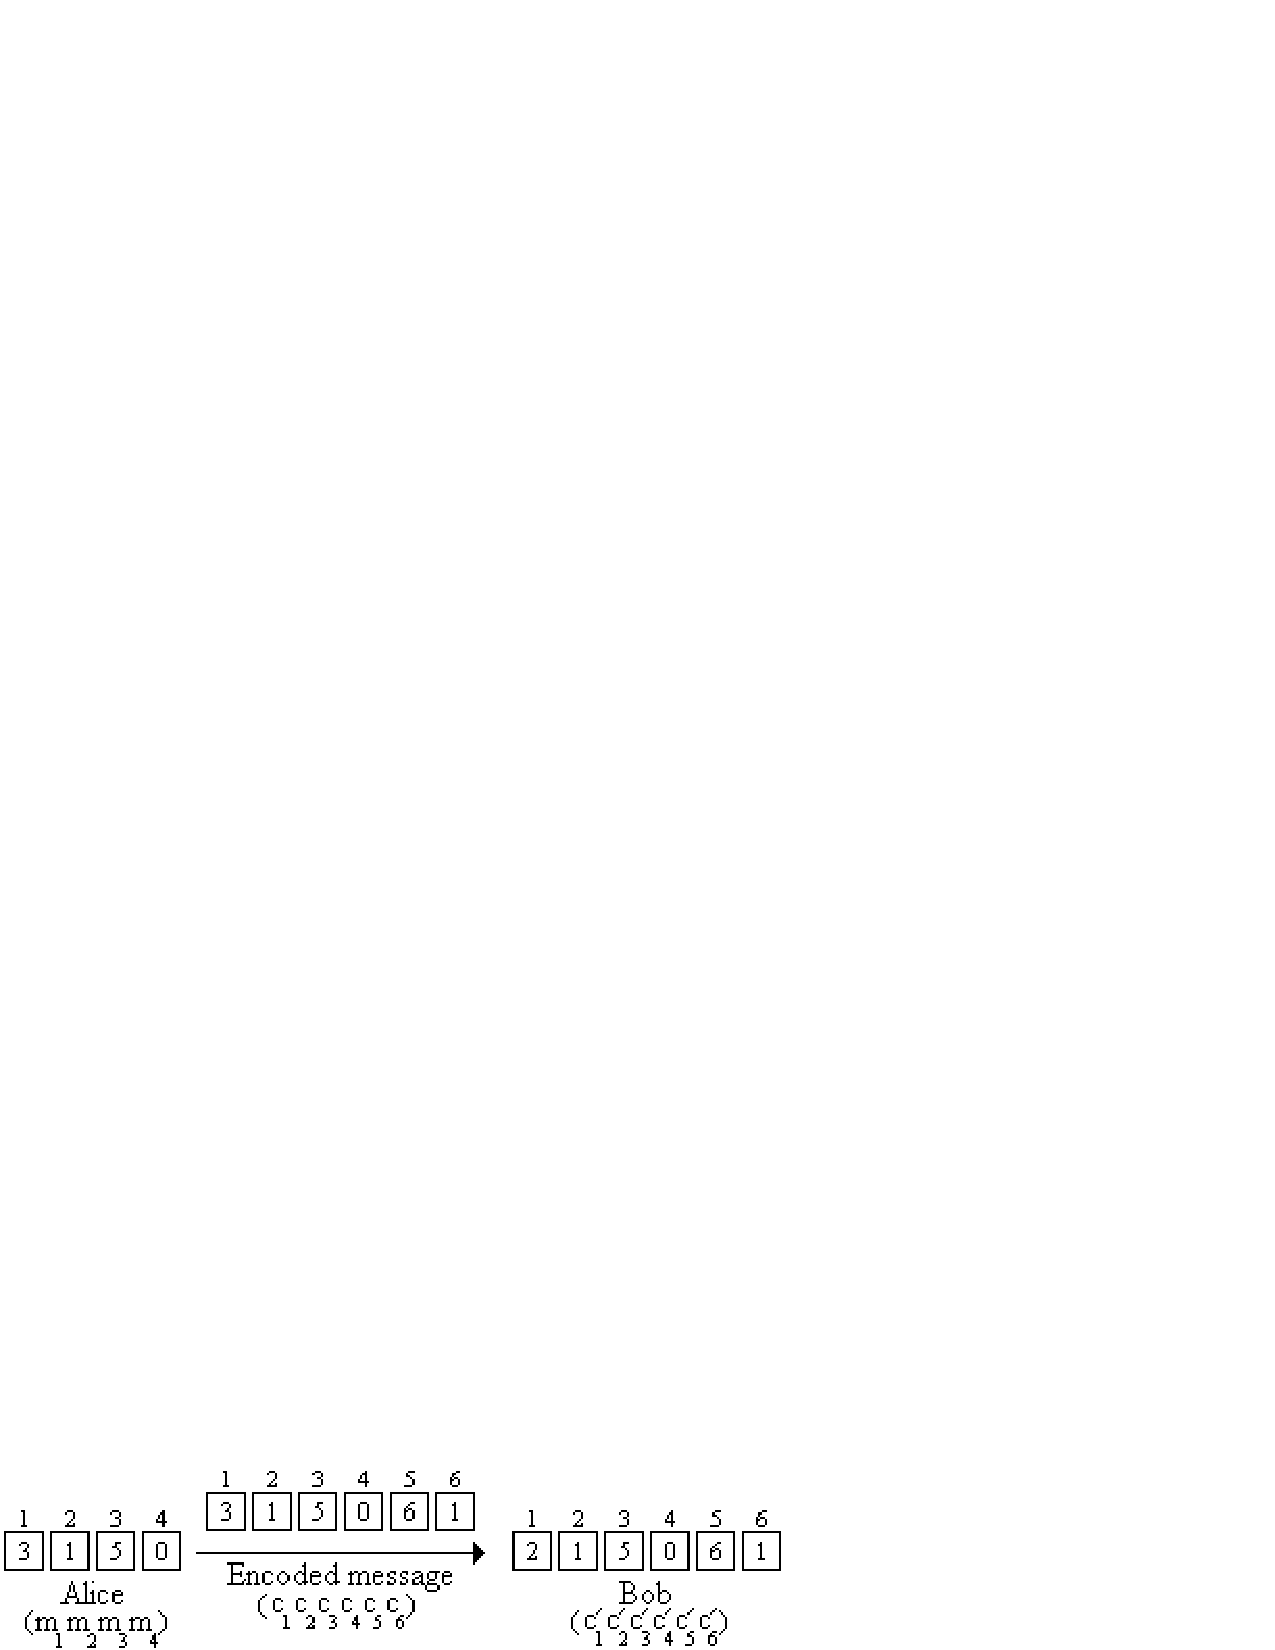
\includegraphics[bb = 0 0 250 87, scale = 0.8]{packets3}

Bob's goal is to reconstruct $P(x)$ from the $n+2k$ received characters
$r_1,\cdots,r_{n+2k}$. He knows that $P(i)$ must equal $r_i$ on at least $n+k$ points (since only $k$ points 
are corrupted), but he does not know which of the $n+k$ values are correct. As an example, 
consider a possible scenario depicted in the 
picture below- the points represent the message received from Alice, and the line represents $P(x)$. 
In this example, $n = 3$, $k = 1$,
and the third packet is corrupted. Bob does not know
the index at which the message and the polynomial deviate: 

\begin{center}
\includegraphics*[scale=0.60]{generalex.png}
\end{center}

Bob attempts to construct $P(x)$ by searching for a polynomial $P'(x)$ with the following property: 
$P'(i) = r_i$ for at least $n+k$ distinct values of $i$ between $1$ and $n+2k$. 
Of course, $P(x)$ is one such polynomial. It turns out that $P(x)$ is actually the only polynomial with
the desired property. Therefore, $P'(x)$ must equal $P(x)$.

Finding $P(x)$ efficiently requires a remarkable idea,
which is just about simple enough to be described here. 
Suppose packets $e_1,\dots,e_k$ are corrupted.
Define the degree $k$ polynomial $E(x)$ to be
$(x-e_1)\cdots(x-e_k)$. 
Let us make a simple but crucial observation: 
$P(i)E(i) = r_iE(i)$ for $1 \leq i \leq n+2k$ 
(this is true at points $i$ at which no
error occurred since $P(i) = r_i$, and trivially 
true at points $i$ at which an error occurred since $E(i) = 0$). 

This observation forms the basis of a very clever 
algorithm invented by Berlekamp and Welch. 
Looking more closely at these equalities, we will show 
that they are $n+2k$ linear equations in $n+2k$ unknowns.
The unknowns correspond to the coefficients of $E(x)$ and $Q(x)$ (where
we define $Q(x) = P(x)E(x)$). Once $Q(x)$ and $E(x)$
are known, we can divide $Q(x)$ by $E(x)$ to obtain $P(x)$. 

Since $Q(x)$ is a polynomial
of degree $n+k-1$, it can be described by $n+k$ coefficients. $E(x)$ is a
degree $k$ polynomial, but its definition implies that its first coefficient must be 1.
It can therefore be described by $k$ coefficients: 
\begin{align*}
Q(x) = a_{n+k-1}x^{n+k-1} + \cdots + a_1x + a_0 \\
E(x) = x^k + b_{k-1}x^{k-1} + \cdots + b_1x + b_0
\end{align*}
As seen in the interpolation method above, once we fix a value $i$ for $x$,
$Q(i)$ and $E(i)$ are linear functions of $a_{n+k-1},\cdots,a_0$ and $b_{k-1},\cdots,b_0$ respectively.
The received value $r_i$ is also fixed. Therefore the equation 
\iffalse
Once we substitute a value $i$ for $x$, where $1 \leq i \leq n+2k$, and the received 
value $r_i$, the equation 
\fi
$Q(i) = r_iE(i)$ is a linear equation in the $n+2k$ 
unknowns $a_{n+k-1}, \ldots, a_0$ and $b_{k-1}, \ldots, b_0$. 
We thus have $n+2k$ linear equations, one for each value of $i$,
and $n+2k$ unknowns.
We can solve these equations and get $E(x)$ and $Q(x)$. 
We can then compute the ratio $\frac{Q(x)}{E(x)}$ to obtain $P(x)$.





%%%% Example

\subsubsection*{Example}

Suppose we are working over $GF(7)$ and Alice wants to send Bob
the $n = 3$ characters ``3,'' ``0,'' and ``6'' over a modem. Turning to the analogy of the English alphabet, this is equivalent to using only the first 7 letters of the alphabet, where $a = 0, b = 1, \ldots, g = 6$. So the message which Alice
wishes for Bob to receive is ``dag''. Then Alice interpolates to
find the polynomial
\[
P(x) = x^2 + x + 1,
\]
which is the unique polynomial of degree $2$ such that $P(1) = 3$,
$P(2) = 0$, and $P(3) = 6$.

Suppose that $k = 1$ character is corrupted, so she needs to transmit the $n + 2k = 5$ characters
$P(1) = 3$, $P(2) = 0$,
$P(3) = 6$, $P(4) = 0$, and $P(5) = 3$ to Bob. Suppose $P(1)$ is corrupted,
so he receives $2$ instead of~$3$ (i.e., Alice sends the encoded message ``dagad'' but Bob instead receives ``cagad''). Summarizing, we have the
following situation:

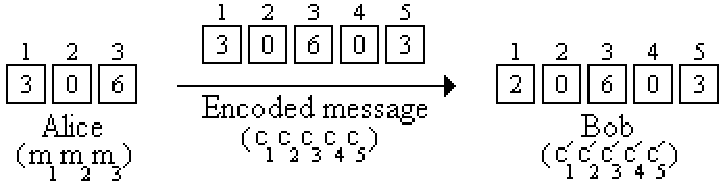
\includegraphics[bb = 0 0 250 90, scale = 0.8]{packets4}

\noindent Let $E(x) = x + b_0$ be the error-locator polynomial---remember, Bob doesn't know
what $b_0$ is yet since he doesn't know where the error occurred. Let $Q(x) = a_3x^3 + a_2x^2 + a_1x + a_0$. 
Now Bob just substitutes $x = 1, x = 2, \cdots, x = 5$ into $Q(x) = r_xE(x)$ and simplifies to get five 
linear equations in five unknowns. Recall that we are working modulo 7 and that $r_i = c_i'$ is the value
Bob received for the $i$-$th$ character. 

The first equation will be $a_3 + a_2 + a_1 + a_0 = 2(1 + b_0)$, which simplifies to
$a_3 + a_2 + a_1 + a_0 + 5b_0 = 2$. Bob can determine the remaining equations in the same manner,
obtaining: 



\iffalse
Then clearly
\[
P(x)E(x) = R(x)E(x)
\]
for $x = 1, 2, \ldots, 5$ (if the corruption occured at position $i$,
then $E(i) = 0$, so equality trivially holds, and otherwise $P(i) =
R(i) = c'_i$). Bob doesn't know what $P$ is (though he does know it is a degree
$2$ polynomial) and he doesn't know what $E$ is either, but using
the relationship above he can obtain a linear system whose solutions
will be the coefficients of $P$ and $E$, as seen below.

Let
\[
Q(x) = a_3x^3 + a_2x^2 + a_1x + a_0 = P(x)E(x),
\]
where $a_3, a_2, a_1, a_0$ are unknown coefficients (which Bob will soon try to
determine), so
\[
a_3x^3 + a_2x^2 + a_1x + a_0 = R(x)E(x) = R(x)(x - e_1),
\]
which he can rewrite as
\[
a_3x^3 + a_2x^2 + a_1x + a_0 + R(x)e_1 = R(x)x.
\]
\fi

\begin{align*}
a_3 + a_2 + a_1 + a_0 + 5b_0 &= 2 \\
a_3 + 4a_2 + 2a_1 + a_0 &= 0 \\
6a_3 + 2a_2 + 3a_1 + a_0 + b_0 &= 4 \\
a_3 + 2a_2 + 4a_1 + a_0 &= 0 \\
6a_3 + 4a_2 + 5a_1 + a_0 + 4b_0 &= 1
\end{align*}
Bob then solves this linear system and finds that $a_3 = 1,$ $a_2 = 0,$ $a_1 = 0,$
$a_0 = 6,$ and $b_0 = 6$ (all mod~7). (As a check, this implies that $E(x)=x+6=x-1$,
so the location of the error is position $e_1=1$, which is correct since
the first character was corrupted from a ``d'' to a ``c''.)  This gives
him the polynomials $Q(x) = x^3 + 6$ and $E(x) = x - 1$. He can then find $P(x)$ by
computing the quotient $P(x) = \frac{Q(x)}{E(x)} = \frac{x^3 + 6}{x - 1} = x^2 + x + 1$. Bob
notices that the first character was corrupted (since $e_1 = 1$), so now that he has $P(x)$, he
just computes
$P(1) = 3 =$ ``d'' and obtains the original, uncorrupted message ``dag''.

%%%% End Example



\subsubsection*{Finer points}
Two points need further discussion. How do we know that the $n + 2k$
equations are consistent? What if they have no solution? 
This is simple. The equations must be consistent since 
$Q(x) = P(x)E(x)$ together with the error
locator polynomial $E(x)$ gives a solution.

A more interesting question is this: how do we know that the $n +
2k$ equations are independent, i.e., how do we know that there
aren't other spurious solutions in addition to the real solution 
that we are looking for? Put more mathematically, how do we know that the solution
$Q'(x)$ and $E'(x)$ that we reconstruct satisfies the property that
$E'(x)$ divides $Q'(x)$ and that $\frac{Q'(x)}{E'(x)} =
\frac{Q(x)}{E(x)}= P(x)$? 

We claim that $Q(x)E'(x) = Q'(x)E(x)$ for $1\leq x\leq n + 2k$. Since the degree of both
$Q(x)E'(x)$ and $Q'(x)E(x)$ is $n + 2k  - 1$ and they are equal at $n + 2k$ points, it follows from Property 2
of Note 7 that
they are the same polynomial. Rearranging, we get $\frac{Q'(x)}{E'(x)} =
\frac{Q(x)}{E(x)}= P(x)$.

Why is the claim above true? Based on our method of obtaining $Q'(x)$ and
$E'(x)$, we know that $Q'(i) = r_iE'(i)$ and $Q(i) = r_iE(i)$. Now assume $E(i)$ is 0. Then
$Q(i)$ is also 0, so both $Q(i)E'(i)$ and $Q'(i)E(i)$ are 0 and the claim holds. The same reasoning applies when
$E'(i)$ is 0. If both $E(i)$ and $E'(i)$ are not 0, we can rearrange the above equality to obtain
$\frac{Q'(i)}{E'(i)} = \frac{Q(i)}{E(i)}$, which implies the claim. 


\end{document}

